%
%
\chapter{Computation of the Static Susceptibility}
\label{appch: static susceptibility}
%
%
In this appendix, the static susceptibility $\chi_{\mt{JP}}(\omega=0)$ is explicitely calculated.
The temperature dependence of $\chi_{\mt{JP}}$ is expected to be non-existent, since momentum and current are not explicitly time dependent.
Using equation \eqref{eq:relation between C, Phi and chi}, the static susceptibility is directly proportional to the Kubo relaxation function \eqref{eq:Kubo relaxation function} at $t=0$.
%
\begin{align}
	\chi_{\mt{PJ}}(\omega = 0) = \Phi_{\mt{PJ}}(t = 0) = i \int\limits_{0}^{\infty} \dd{t'} \expval{\comm{\mt{P}_{j}(t')}{\mt{J}_{j}(0)}}
\end{align}
%
In the formula above, the limit $s\to0$ is dropped, since the integral is assumed to be convegent.
The spatial direction of P and J is signified by the index $j$.
The integral is transformed into Matsubara time $\tau = it$, firstly.
The Jacobi determinate is $-i$ and the integral's limits is set to $0$ and $\beta$.
Observing only the zeroth order in pertubation theory the static susceptibility is given by
%
\begin{align}
	\chi_{\mt{PJ}}(\omega = 0) = \int\limits_{0}^{\beta} \dd{\tau} \expval{\mathcal{T}_{\tau} \mt{P}_{j}(\tau) \mt{J}_{j}(0)}_{0}.
\end{align}
%
The momentum and current operators are named in equation \eqref{eq:momentum operator} and \eqref{eq:current operator}, respetivily.
Inserting them, expectation values are generated including four operators.
Only if these operators are of the same species, $\Phi_{\mu}$, $\Psi_{\mt{a}}$ or $\Psi_{\mt{b}}$, the expectation values yield connected diagrams.
This happens two times in the case of fermionic operators.
%
\begin{figure}[t]
	\centering
	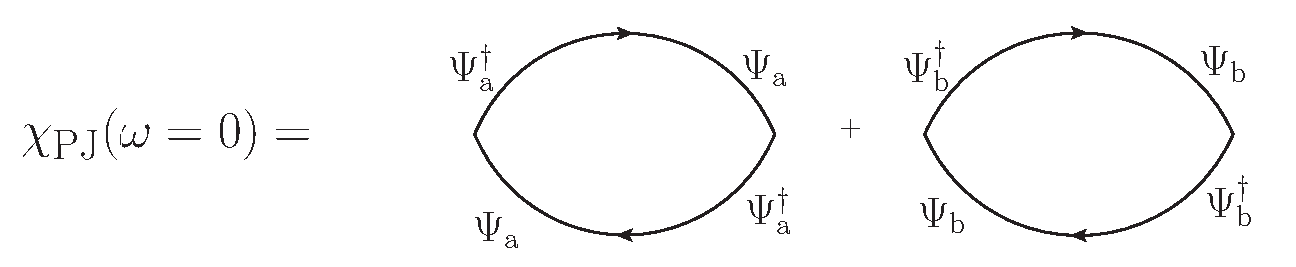
\includegraphics[width=0.8\textwidth]{static_susceptibility.eps}
	\caption{caption}
	\label{fig:static susceptibility}
\end{figure}
%
Wick's theorem is used to seperate the remaining two expectation values in terms of free Green functions.
The contraction of operators with different time argument is generated the two bubble diagrams, depicted in figure \ref{fig:static susceptibility}
The static susceptibility is given by
%
\begin{align}
	\chi_{\mt{PJ}}(\omega = 0) &= 
		\int\limits_{0}^{\beta} \dd{\tau} 
		\int_{\vb{k}} 
		k_{j}^{2}
		\bigg[
			\frac{1}{m_{1}}
			\mathcal{G}_{\mt{a}}^{(0)}(\vb{k},-\tau)
			\mathcal{G}_{\mt{a}}^{(0)}(\vb{k},\tau)
			+
			\frac{1}{m_{2}}
			\mathcal{G}_{\mt{b}}^{(0)}(\vb{k},-\tau)
			\mathcal{G}_{\mt{b}}^{(0)}(\vb{k},\tau)
		\bigg].
\end{align}
%
Here the free fermionic propagator $\mathcal{G}_{\alpha}^{(0)}(\vb{k},\tau) = -\expval*{\mathcal{T}_{\tau} \Psi_{\alpha}(\vb{k},\tau) \Psi_{\alpha}^{\dag}(\vb{k},0)}$ with $\alpha \in \{\mt{a},\mt{b}\}$ is inserted.
Both fermionic Green functions are transformed into the Matsubara frequency space.
The only $\tau$-dependence is thus given by the exponential functions.
The $\tau$-integral is evaluated, using the definition of the $\delta$-distribution in Matsubara space, $\int_{0}^{\beta} \dd{\tau} \exp(i(\omega_{m} - \omega_{n})\tau) = \beta \delta(\omega_{m} - \omega_{n})$.
One of the two sums over Matsubara frequencies is easily performed due to this $\delta$-distribution.
The obtained expression is given by
%
\begin{align}
	\chi_{\mt{PJ}}(\omega = 0) &= 
		\frac{1}{\hbar} 
		\int_{\vb{k}} 
		k_{j}^{2}
		\bigg[
			\frac{1}{m_{1}}
			S_{\mt{a}}(\omega_{n})
			+
			\frac{1}{m_{2}}
			S_{\mt{b}}(\omega_{n})
		\bigg].
\end{align}
%
The Matsubara sum $S_{\alpha}(\omega_{n}) = \beta^{-1} \sum_{\omega_{n}} \mathcal{G}_{\alpha}^{(0)}(\vb{k},\omega_{n}) \mathcal{G}_{\alpha}^{(0)}(\vb{k},\omega_{n})$, where $\alpha = \mt{a}, \mt{b}$, is defined.
This sum is transformed into a complex contour integral, offering the use of the usual complex analysis.
The product of Green functions multiplied with the Fermi distribution are generated the integrand of this contour integral.
The full transformation rule is given by
%
\begin{align}
	S = \frac{1}{\beta} \sum\limits_{\omega_{n}} \mathcal{G}(\omega_{n}) = -\frac{1}{2\pi i} \oint_{\Gamma} \dd{z} n_{\mt{F}}(z) \mathcal{G}(z).
\end{align}
%
The choice of the contour is arbitrary beside one condiction.
All singularies of the Green functions are excluded in the contour, while the infinite poles $\omega_{n} = \flatfrac{(2n+1)\pi}{\beta}$, where $n\in\mathbb{Z}$, of the Fermi distribution are included in the contour.
Our starting contour $\Gamma$ is depicted on the left hand side in figure \ref{fig:contour simple poles}.

The contour is generated by to path along the imaginary axis, from $i\infty$ to $$-i\infty$ and vice versa.
Both paths are connected in plus and minus infinity and shifted infinitesimal aside the imaginary axis.
This contour is now expaned to a circle with radius infinity, where always the singularities of the Green function is excluded.
The obtained contour is depicted on the right hand side in figure \ref{fig:contour simple poles}.
The same magnitude with opposite sign is generated by the paths from infinity to the poles and vice versa.
Therefore, the contour is seperated into small circles around the poles of the Green functions and into one circle with infinite radius.
The contribution of the latter is zero, since the Green function is proportional to $\flatfrac{1}{z}$.
In the remaining contour integrals the product of Green functions is now inserted, where the single free fermionic Green function is given by
%
\begin{figure}[t]
	\centering
	\includegraphics[width=0.8\textwidth]{contour_simple_poles.pdf}
	\caption{caption}
	\label{fig:contour simple poles}
\end{figure}
%
%
\begin{align}
	\mathcal{G}_{\alpha}(\vb{k}, i\omega_{n}) = \frac{1}{i\omega_{n} - \epsilon_{\alpha}(\vb{k})}.
\end{align}
%
$\epsilon_{\alpha}(\vb{k})$, where $\alpha = \mt{a},\mt{b}$, is the fermion's dispersion and also the singularity of the Green function.
The explicite expression is denoted in equation \eqref{eq:dispersion relations}.
Besides this singularity, the Green function is holomoph in the whole complex plane.
The contour integral is evaluated using the resiuum theorem, which yields
%
\begin{align}
	\chi_{\mt{PJ}}(\omega = 0) &= 
		- \int_{\vb{k}} 
		k_{j}^{2}
		\bigg[
			\frac{1}{m_{1}}
			\dv{n_{\mt{F}}(\epsilon_{\mt{a}}(\vb{k}))}{\epsilon_{\mt{a}}(\vb{k})}
			+
			\frac{1}{m_{2}}
			\dv{n_{\mt{F}}(\epsilon_{\mt{b}}(\vb{k}))}{\epsilon_{\mt{b}}(\vb{k})}
		\bigg]
\end{align}
%
The derivatives of the distribution function with respect to the dispersion relation are generated, since the integrand has a singularity of second order at $z_{0} = \epsilon_{\alpha}(\vb{k})$.
These two obtained integrals are exactly solvable.
Therefore the inetegrals are transformed into plane polar coordinates, where the transformation rule is given by $(k_{x}, k_{y}) = (q\sqrt{2m_{1,2}}\cos(\phi), q\sqrt{2m_{2,1}}\sin(\phi))$.
Two typs of transformation are used, since the dispersion relation of the two species of fermions differs in the contained mass terms.
The only angular dependece is originated by the $k_{j}^{2}$-term.
This term yields $\cos[2](\phi)$ or $\sin[2](\phi)$ for the $x$- or $y$-direction, respectivily.
Since the limits of the $\phi$-integral are $0$ and $2\pi$, the contribution is $\pi$ in both cases.
The upper limit of the $q$-integral is set to infity, since the integrand is decreasing fast to zero for large values of $q$.
%
\begin{align}
	\chi_{\mt{PJ}}(\omega = 0) = 
		\frac{8 \beta \pi}{(2\pi)^{2}} \sqrt{m_{1} m_{2}}
		\int\limits_{0}^{\infty} \dd{q}
		q^{3} \frac{e^{\beta(q^{2} - \mu)}}{(e^{\beta(q^{2} - \mu)} + 1)^{2}}
\end{align}
%
The obtained integral is solved, substituting $x = \beta(q^{2} - \mu)$.
The first of the two obtained integrals is evaluated using integration by parts, while the derivative of the Fermi distribution with respect to $x$ is originated in the second integral.
Performing these integrals the static susceptibility of J and P is given by
%
\begin{align}
	\chi_{\mt{PJ}}(\omega = 0) = \frac{\sqrt{m_{1} m_{2}}}{\pi \beta}\ln(e^{\beta \mu} + 1)
\end{align}
%
In the case of $\mu \gg k_{\mt{B}} T$, the exponential function is large compared to 1 and neglectable.
The static susceptibility is then temperature independent in the leading order and given by
%
\begin{align}
	\chi_{\mt{PJ}}(\omega = 0) \to \frac{\mu \sqrt{m_{1} m_{2}}}{\pi} \qquad (T \to 0)
\end{align}
%